\section{Approach}
\label{sec:approach}
In this section, we discuss how a mention in Web table is mapped to an entity in KB. Given a Web table in language $A$ and a KB in language $B$, we firstly generate a list of candidate entities in language $B$ for each mention, then find the target entity among them. Due to the language gap and characteristic of tables, we propose a jointly modeling framework using nerual networks.

%\subsection{Model Overview}

In this section, we describe our joint model for cross-lingual table linking.
%\figref{fig:overview} gives a general view of our neural network based joint model.
\figref{fig:overview} gives a general view of the model.
The reason we call it a ``joint model'' is that
the input of neural network is a mention table $X$ containing all the cells to be linked,
together with one candidate entity table $E$,
%All the mentions in the table will be linked simultaneously.
and the output stands for the relevance score $S(X, E)$.
%which indicates the probability of choosing that candidate entity table as final result.

Specifically, we first generate candidate entities of each single mention (\secref{sec:candgen}),
then we learn two different features:
the \textbf{m}ention feature and \textbf{c}ontext feature
derived from the mention-entity embedding pairs of the table (\secref{sec:cell}).
To make different representations from two language spaces compatible,
we utilize a bilingual translation matrix to transform the vector representation
from Chinese to English (\secref{sec:translation}).
Meanwhile, we learn a third feature called \textbf{coh}erence feature
only from the candidate entity table (\secref{sec:coherence}).
%We combine these three features together to calculate the overall relevance score, and finally
Finally, we discuss the prediction and parameter learning step of this task (\secref{sec:strategy}). 

\begin{figure*}
	\centering
	%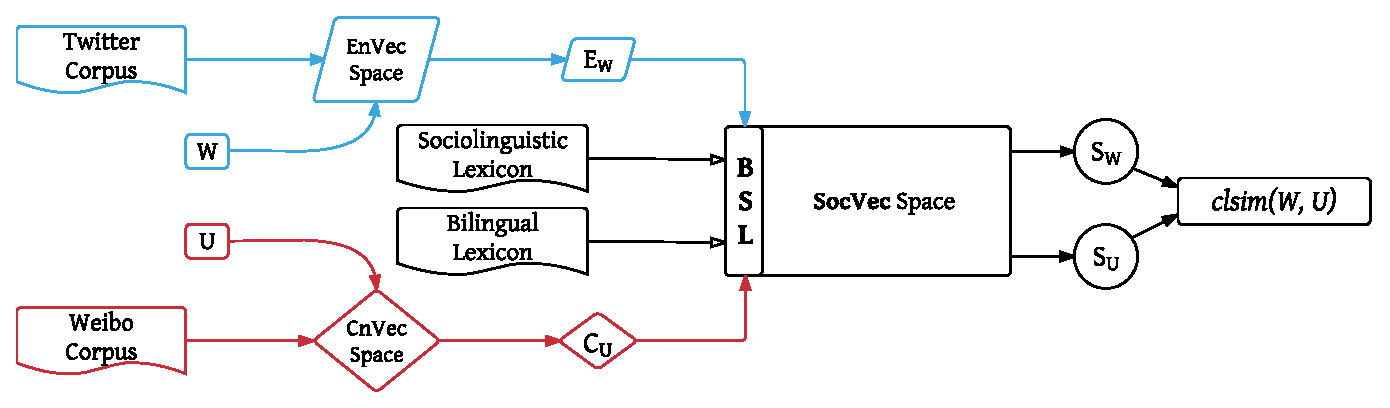
\epsfig{file=figures/overview.eps, angle=0, width=2.0\columnwidth}
	\scalebox{0.28}{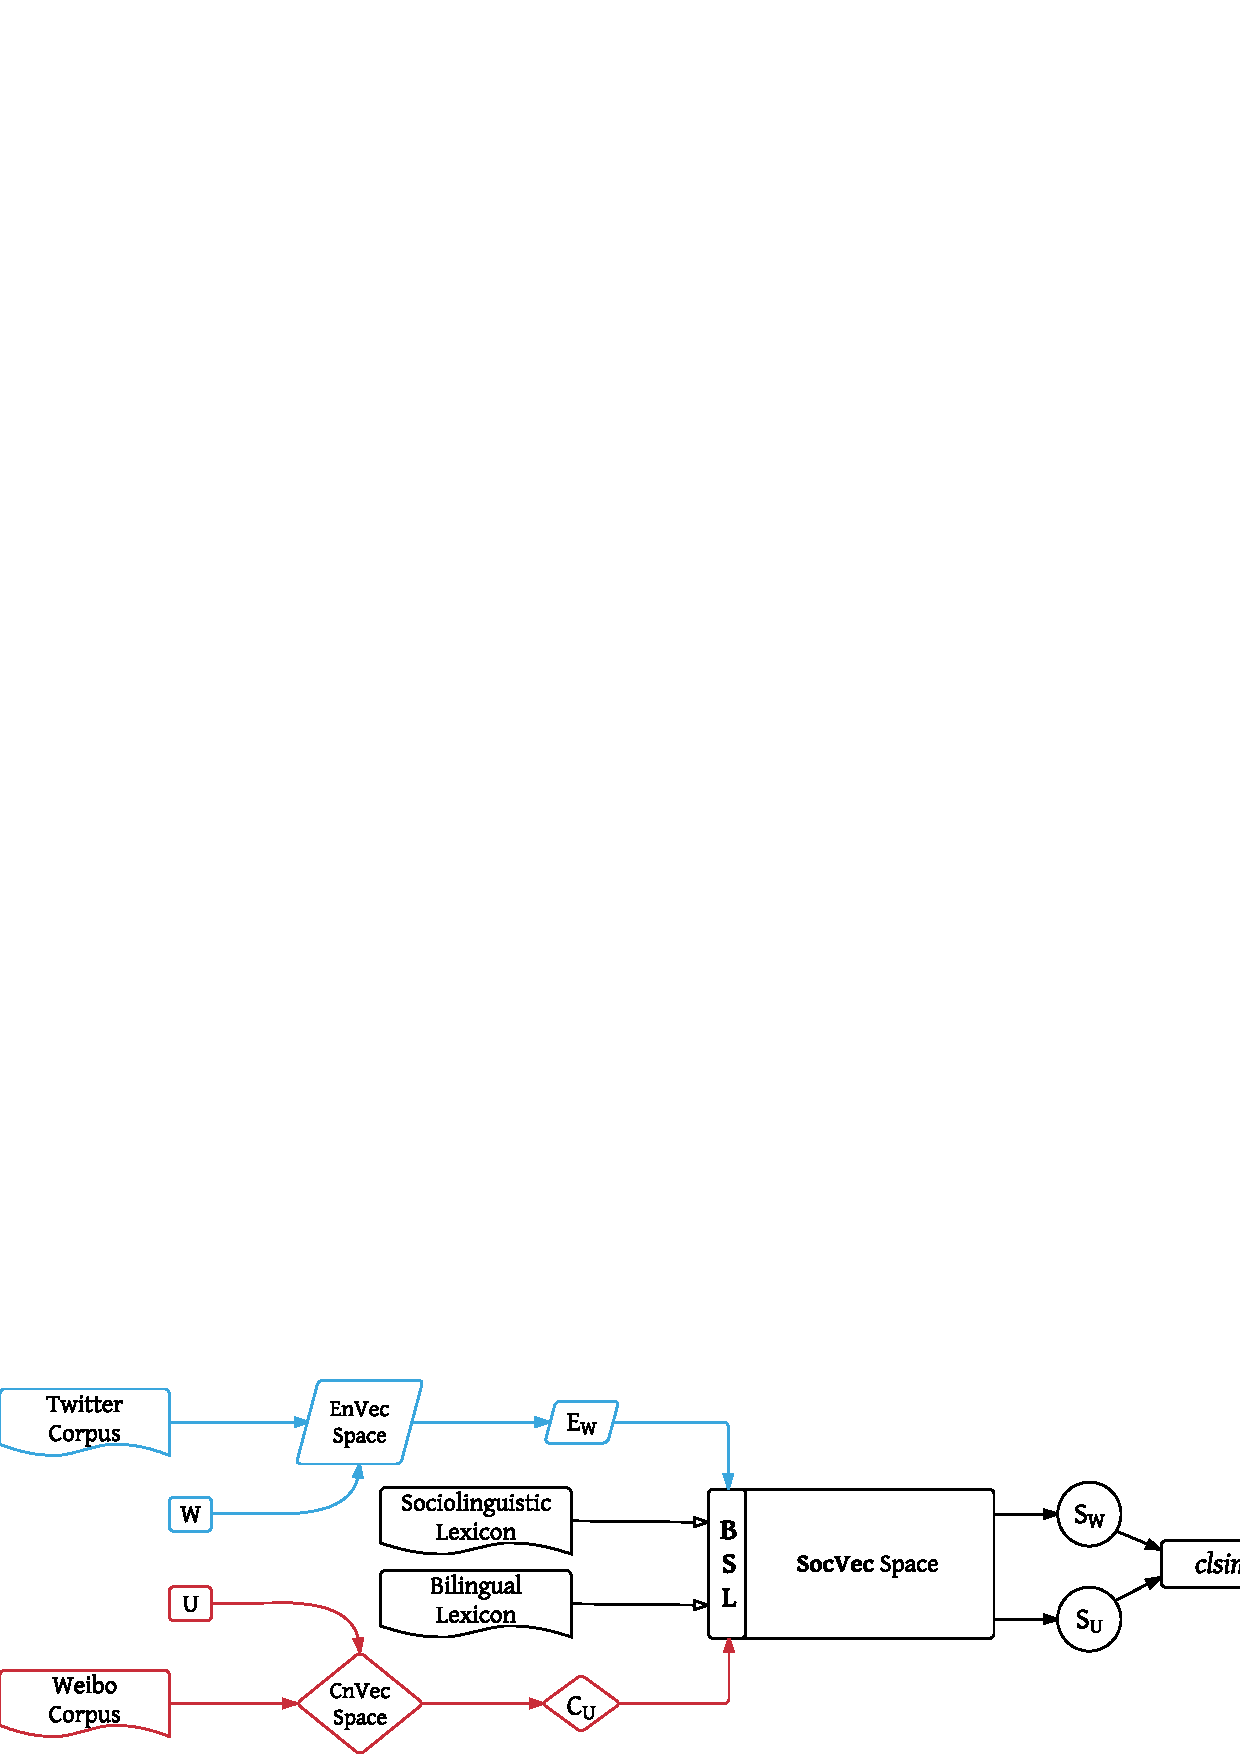
\includegraphics{figures/overview.pdf}}
	\caption{Overview of proposed neural network based joint model.}
	\label{fig:overview}
\end{figure*}


\input{surfaceFeature}
\input{contextFeature}
\subsection{Coherence Feature}
\label{sec:coherence}

The previous two features aim at
encoding the relevance or compatibility of the mention-entity table pair.
On the other hand,
the inner relationship of entities in the correct linked table is also valuable.
The intuition is that entities in the same column (row) tend to own the 
same type, in which case, lead to similar vector representations.
In the example in \figref{fig:chinesetable}, target entities of 
the three columns
represent ``university'', ``street'' and ``city'', respectively.
%or we can say that their embeddings are very close.
Therefore, we propose a third feature,
which captures such correlations among entities of same column. 

%\KZ{How do you distinguish between columns and rows?  Some tables have same-type columns, while others have same-type rows.}
%\XS{Cite papers doing table type classification, where one of those table types (6 in total) is called Vertical Relational (VR), which is exactly the format of tables in our experiments. We could say we just choose to focous this type of tables, and one can use those classifiers to unify table formats into VR and then use our model to do entity linking. }

There have been several works~\cite{eberius2015building,nishida2017understanding} on table type classification,
which identifies the display form of web tables.
In this paper, we mainly focus on tables with type 
``Vertical Relational'' (VR) \cite{nishida2017understanding},
which just look like \figref{fig:chinesetable}, where entities in the 
same column have the same type.
Most of web tables can be transformed into this type after classification, 
which is outside the scope of this paper.

We calculate the element-wise variance for all entity vectors in the same column
to get a coherence vector for that column.
The average among all columns is the hidden \textbf{coh}erence feature
$\bi{h}^{(coh)}$ of whole entity table:

\begin{equation}
  \label{eqn:coherence}
    \bi{h}^{(coh)} = \frac{1}{C} \sum_{j} \bi{var}(\{\bi{e}_{ij} | (i,j) \in P \}),
\end{equation}
\noindent
where $\bi{var}(\cdot)$ calculates element-wise variance for a bunch of 
input vectors.
The coherence feature captures how self-organized the candidate entities are,
which complements the previous mention and context features.

